\documentclass{article}
\usepackage{titlesec}
\usepackage[utf8]{inputenc}
\usepackage[a4paper, total={6in, 9in}]{geometry}
\usepackage{fancyhdr}
\usepackage{graphicx} % Add the graphicx package
\usepackage{lipsum} % For placeholder text
\usepackage{tikz}

\usepackage[hidelinks]{hyperref}
\usepackage{wrapfig}
\usepackage{acronym}
\usepackage{float}
\usepackage{multicol}
\usepackage{bm}
\usepackage{circuitikz}
\usetikzlibrary{shapes.geometric}
\usepackage{caption}
\usepackage{acronym}
\usepackage{amsmath,amssymb,amsfonts}
\usepackage{algorithmic}
\usepackage{textcomp}
\usepackage{xcolor}
\usepackage[numbers]{natbib}
\bibliographystyle{ieeetran}
\usepackage{url}
% Set up page headers and footers
\pagestyle{fancy}
\fancyhf{}
\rhead{Electro Dieus}
\lhead{\textit{Five Band Audio Equalizer}}
\cfoot{\thepage}

% Redefine the abstract environment to be single column
\renewenvironment{abstract}
{\par\noindent\textbf{\abstractname}\ \ignorespaces}{\par}

% Redefine section format
\titleformat{\section}
{\normalfont\Large\bfseries}{\thesection}{1em}{}

\begin{document}
	
	% Cover Page
	\begin{titlepage}
		
		\centering
		\vspace*{0.5cm}
		\includegraphics[width=5cm]{University_of_Moratuwa_logo.png} % Replace with the path to your university logo
		\par\vspace{0.02cm}
		{\fontfamily{lmss}
			{\Large Department of Electronic \& Telecommunication Engineering,\\
				University of Moratuwa, Sri Lanka.}}
		\par\vspace{2cm}
		{\LARGE\bfseries Five Band Audio Equalizer\par}
		\vspace{6cm}
		{\large Group Members:\par}
		\begin{tabular}{l l}
			
			230629R	&	Tennakoon U.G.R.B\\
			230548R 	&	Ratnayake R.M.S.H\\
			230613M	&	Shehan M.N.N \\
			230164K	&	Dissanayake R.K.T\\
			
		\end{tabular}\\
		\vspace{1.5cm}
		{Submitted in partial fulfillment of the requirements for the module\par}
		{EN 2091 Laboratory Practice and Projects\par}
		
		\vspace{1.0cm}
		{ Date: \today}
		\vfill
	\end{titlepage}
	
	\newpage
	
	% Abstract
	\begin{abstract}
		\\
		The \textbf{Five Band Audio Equalizer} is an analog signal processing system designed to modify and enhance audio quality by adjusting the amplitude of distinct frequency bands within an audio signal. The system divides the input audio into five specific frequency ranges---20--300~Hz, 300~Hz--1~kHz, 1--4~kHz, 4--10~kHz, and 10--20~kHz---using precision-designed band-pass filters. Each band can be individually amplified or attenuated through a variable gain control stage, enabling users to shape the tonal balance according to preference or acoustic environment. A preamplifier circuit prepares the signal for processing, while a summing amplifier recombines the adjusted frequency bands to produce a clear and balanced output. Additionally, an \ac{LED}-based level display visually indicates the intensity of each band. The system is implemented using operational amplifiers (NE5532) and the LM3915 display driver, ensuring low noise, high fidelity, and efficient visualization. This project demonstrates practical applications of analog circuit design principles, including filter design, signal amplification, \ac{PCB} layout, and system integration for real-world audio enhancement.
		
	\end{abstract}
	\section*{Abbreviations and Acronyms}
	\begin{acronym}
		\acro{PCB}{Printed Circuit Board}
		\acro{Op Amp}{Operational Amplifier}
		\acro{LED}{Light Emitting Diode}
		\acro{MFB}{Multiple Feedback}
	\end{acronym}
	\newpage
	% Table of Contents
	\tableofcontents
	\newpage
	
	% Sections
	\section{Introduction and Functionality}
	An \textbf{audio equalizer} is a fundamental device used in sound systems to balance and adjust the amplitude of specific frequency components within an audio signal. It enables selective amplification or attenuation of chosen frequency ranges, thereby enhancing tonal quality and the overall listening experience. 
	
	In this project, a \textbf{Five Band Audio Equalizer} was developed using analog electronic circuits to divide the incoming audio signal into five distinct frequency bands:
	\begin{itemize}
		\item 20--300~Hz (Bass range)
		\item 300~Hz--1~kHz (Lower midrange)
		\item 1--4~kHz (Upper midrange)
		\item 4--10~kHz (Presence range)
		\item 10--20~kHz (Treble range)
	\end{itemize}
	
	20-300 Hz frequency band is processed using an unity gain Sallen-Key band-pass filter and other frequency bands processed through \ac{MFB} filter to isolate its respective range. The filtered signals then pass through individual \textbf{gain control stages}, allowing users to adjust amplification levels via variable resistors. The processed signals are subsequently recombined using a \textbf{summing amplifier} to produce a customized and balanced output signal.
	
	A \textbf{pre-amplifier} boosts the input audio signal to the required level, while a \textbf{power amplifier} (based on the LM386 IC) drives the final output with sufficient power. Furthermore, a \textbf{\ac{LED} level indicator} circuit, implemented using the LM3915 \ac{LED} display driver, provides real-time visual feedback of the audio levels across frequency bands. 
	
	Overall, this system integrates the concepts of \textbf{analog filtering}, \textbf{amplification}, and \textbf{signal visualization} into a single compact hardware unit, demonstrating the principles of audio signal processing and analog circuit design in a practical and educational context.
	
	
	\section{System Architecture}
	
	\begin{figure}[H]
		\centering
		% Resize to fit page width
		\resizebox{\textwidth}{!}{%
			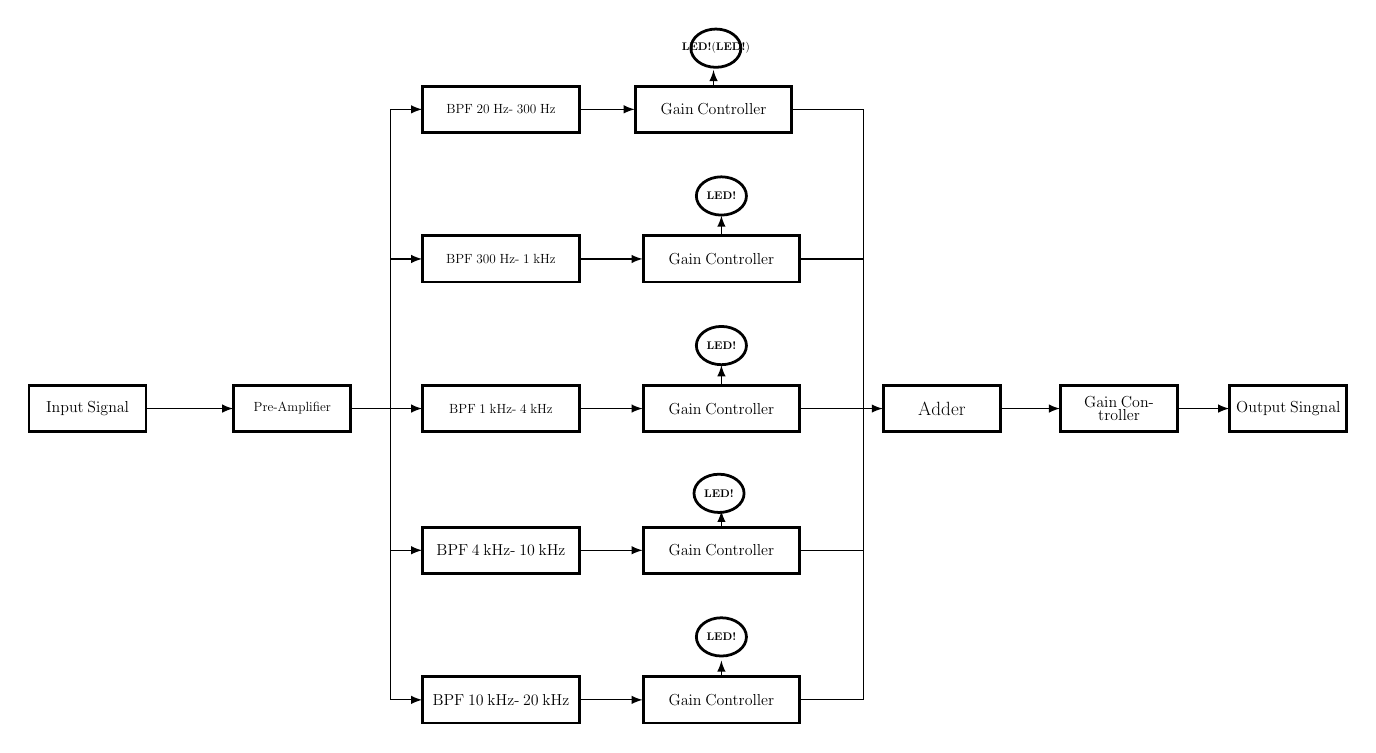
\begin{tikzpicture}[scale=0.4,transform shape]	% Paths, nodes and wires:
				\node[shape=rectangle, draw, line width=1pt, minimum width=3.715cm, minimum height=1.465cm] at (-26.625, 11.75){} node[anchor=center, align=center, text width=3.327cm, inner sep=6pt] at (-26.625, 11.75){\Large Input Signal};
				\node[shape=rectangle, draw, line width=1pt, minimum width=3.715cm, minimum height=1.465cm] at (-20.125, 11.75){} node[anchor=center, align=center, text width=3.327cm, inner sep=6pt] at (-20.125, 11.75){\large Pre-Amplifier};
				\node[shape=rectangle, draw, line width=1pt, minimum width=4.965cm, minimum height=1.465cm] at (-13.5, 21.25){} node[anchor=center, align=center, text width=4.577cm, inner sep=6pt] at (-13.5, 21.25){\large BPF 20 Hz- 300 Hz};
				\node[shape=rectangle, draw, line width=1pt, minimum width=4.965cm, minimum height=1.465cm] at (-13.5, 11.75){} node[anchor=center, align=center, text width=4.577cm, inner sep=6pt] at (-13.5, 11.75){\large BPF 1 kHz- 4 kHz};
				\node[shape=rectangle, draw, line width=1pt, minimum width=4.965cm, minimum height=1.465cm] at (-13.5, 16.5){} node[anchor=center, align=center, text width=4.577cm, inner sep=6pt] at (-13.5, 16.5){\large BPF 300 Hz- 1 kHz};
				\node[shape=rectangle, draw, line width=1pt, minimum width=4.965cm, minimum height=1.465cm] at (-13.5, 7.25){} node[anchor=center, align=center, text width=4.577cm, inner sep=6pt] at (-13.5, 7.25){\Large BPF 4 kHz- 10 kHz};
				\node[shape=rectangle, draw, line width=1pt, minimum width=4.965cm, minimum height=1.465cm] at (-13.5, 2.5){} node[anchor=center, align=center, text width=4.577cm, inner sep=6pt] at (-13.5, 2.5){\Large BPF 10 kHz- 20 kHz};
				\node[shape=rectangle, draw, line width=1pt, minimum width=4.965cm, minimum height=1.465cm] at (-6.75, 21.25){} node[anchor=center, align=center, text width=4.577cm, inner sep=6pt] at (-6.75, 21.25){\Large Gain Controller};
				\node[shape=rectangle, draw, line width=1pt, minimum width=4.965cm, minimum height=1.465cm] at (-6.5, 16.5){} node[anchor=center, align=center, text width=4.577cm, inner sep=6pt] at (-6.5, 16.5){\Large Gain Controller};
				\node[shape=rectangle, draw, line width=1pt, minimum width=4.965cm, minimum height=1.465cm] at (-6.5, 11.75){} node[anchor=center, align=center, text width=4.577cm, inner sep=6pt] at (-6.5, 11.75){\Large Gain Controller};
				\node[shape=rectangle, draw, line width=1pt, minimum width=4.965cm, minimum height=1.465cm] at (-6.5, 7.25){} node[anchor=center, align=center, text width=4.577cm, inner sep=6pt] at (-6.5, 7.25){\Large Gain Controller};
				\node[shape=rectangle, draw, line width=1pt, minimum width=4.965cm, minimum height=1.465cm] at (-6.5, 2.5){} node[anchor=center, align=center, text width=4.577cm, inner sep=6pt] at (-6.5, 2.5){\Large Gain Controller};
				\node[shape=rectangle, draw, line width=1pt, minimum width=3.715cm, minimum height=1.465cm] at (0.5, 11.75){} node[anchor=center, align=center, text width=3.327cm, inner sep=6pt] at (0.5, 11.75){\LARGE Adder};
				\node[shape=rectangle, draw, line width=1pt, minimum width=3.715cm, minimum height=1.465cm] at (6.125, 11.75){} node[anchor=center, align=center, text width=3.327cm, inner sep=6pt] at (6.125, 11.75){\Large Gain Controller};
				\node[shape=rectangle, draw, line width=1pt, minimum width=3.715cm, minimum height=1.465cm] at (11.5, 11.75){} node[anchor=center, align=center, text width=3.327cm, inner sep=6pt] at (11.5, 11.75){\Large Output Singnal};
				\node[shape=ellipse, draw, line width=1pt, minimum width=1.59cm, minimum height=1.215cm](N1) at (-6.675, 23.192){} node[anchor=center] at (N1.text){$\ac{LED}$};
				\node[shape=ellipse, draw, line width=1pt, minimum width=1.59cm, minimum height=1.215cm](N2) at (-6.5, 18.5){} node[anchor=center] at (N2.text){$\ac{LED}$};
				\node[shape=ellipse, draw, line width=1pt, minimum width=1.59cm, minimum height=1.215cm](N3) at (-6.5, 13.75){} node[anchor=center] at (N3.text){$\ac{LED}$};
				\node[shape=ellipse, draw, line width=1pt, minimum width=1.59cm, minimum height=1.215cm](N4) at (-6.575, 9.058){} node[anchor=center] at (N4.text){$\ac{LED}$};
				\node[shape=ellipse, draw, line width=1pt, minimum width=1.59cm, minimum height=1.215cm](N5) at (-6.5, 4.5){} node[anchor=center] at (N5.text){$\ac{LED}$};
				\draw[-latex] (-24.75, 11.75) -- (-22, 11.75);
				\draw[-latex] (-18.25, 11.75) -- (-16, 11.75);
				\draw[-latex] (-17, 11.75) -- (-17, 7.25) -- (-16, 7.25);
				\draw[-latex] (-17, 7.25) -- (-17, 2.5) -- (-16, 2.5);
				\draw[-latex] (-17, 11.75) -- (-17, 16.5) -- (-16, 16.5);
				\draw[-latex] (-17, 16.5) -- (-17, 21.25) -- (-16, 21.25);
				\draw[-latex] (-11, 21.25) -- (-9.25, 21.25);
				\draw[-latex] (-11, 16.5) -- (-9, 16.5);
				\draw[-latex] (-11, 11.75) -- (-9, 11.75);
				\draw[-latex] (-11, 7.25) -- (-9, 7.25);
				\draw[-latex] (-11, 2.5) -- (-9, 2.5);
				\draw[-latex] (-6.5, 3.25) -- (-6.5, 3.75);
				\draw[-latex] (-6.5, 8) -- (-6.5, 8.5);
				\draw[-latex] (-6.5, 12.5) -- (-6.5, 13.125);
				\draw[-latex] (-6.5, 17.25) -- (-6.5, 17.75) -- (-6.5, 17.875);
				\draw[-latex] (-6.75, 22) -- (-6.75, 22.5);
				\draw[-latex] (-4, 11.75) -- (-1.375, 11.75);
				\draw[-latex] (2.375, 11.75) -- (4.25, 11.75);
				\draw[-latex] (8, 11.75) -- (9.625, 11.75);
				\draw (-4, 2.5) -- (-2, 2.5) -- (-2, 11.75);
				\draw (-4, 7.25) -- (-2, 7.25);
				\draw (-4.25, 21.25) -- (-2, 21.25) -- (-2, 11.75);
				\draw (-4, 16.5) -- (-2, 16.5);
			\end{tikzpicture}
		}
		\caption{Functional Block Diagram}
		\label{fig:Functional Block Diagram}
	\end{figure}
	
	
	
	\subsection{Pre-Amplifier Circuit}
	\begin{figure}[H]
		\centering
		% Resize to fit page width
		\resizebox{0.7\textwidth}{!}{%
			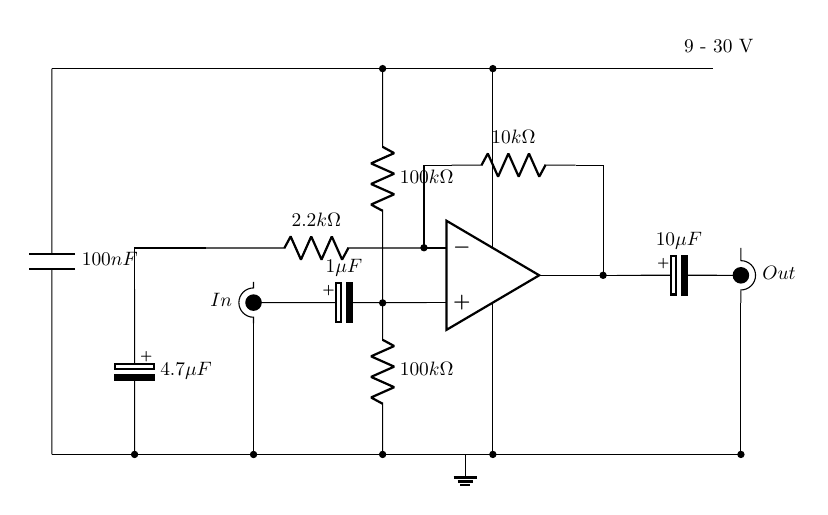
\begin{tikzpicture}[scale=0.7, transform shape]
				
				
				% Paths, nodes and wires:
				\draw (-17, 12) -- (-5, 12);
				\draw (-11, 12) to[american resistor, l={$100 k\Omega$}] (-11, 8);
				\draw (-11, 8) to[american resistor, l={$100 k\Omega$}] (-11, 5);
				\draw (-14.202, 8.745) to[american resistor, l={$2.2 k\Omega$}] (-10.202, 8.745);
				\draw (-17, 12) to[capacitor, l={$100 nF$}] (-17, 5);
				\draw (-17, 5) -- (-5, 5);
				\draw (-15.5, 8) to[ecapacitor, l={$4.7 \mu F$}] (-15.5, 5);
				\draw (-13.202, 7.755) to[ecapacitor, l={$1 \mu F$}] (-10.202, 7.755);
				\node[op amp, xscale=1.01, yscale=1.01] at (-9, 8.25){};
				\draw (-6.75, 8.25) to[ecapacitor, l={$10 \mu F$}] (-4.5, 8.25);
				\draw (-7.75, 8.25) -- (-6.75, 8.25);
				\draw (-7, 8.25) -| (-7, 10.25) -- (-7.5, 10.25);
				\draw (-9.75, 10.25) -- (-10.25, 10.25) -- (-10.25, 8.75);
				\draw (-14.202, 8.745) -| (-15.5, 8);
				\draw (-13.342, 7.38) to[currtap, l={$In$}] (-13.342, 8.13);
				\draw (-4.5, 8.75) to[currtap, l={$Out$}] (-4.5, 7.75);
				\draw (-4.5, 7.75) -| (-4.5, 5) -- (-5, 5);
				\draw (-9, 8.75) -- (-9, 12);
				\draw (-9, 7.75) -| (-9, 5);
				\node[ground] at (-9.5, 5){};
				\node[circ] at (-15.5, 5){};
				\node[circ] at (-13.342, 4.999){};
				\node[circ] at (-11, 5){};
				\node[circ] at (-9, 5){};
				\node[circ] at (-4.5, 5){};
				\node[circ] at (-9, 12){};
				\node[circ] at (-11, 12){};
				\node[circ] at (-11, 7.75){};
				\node[circ] at (-10.25, 8.75){};
				\node[circ] at (-7, 8.25){};
				\draw (-7.798, 8.25) -- (-7.75, 8.25);
				\node[shape=rectangle, minimum width=1.965cm, minimum height=0.465cm] at (-4.75, 12.5){} node[anchor=north west, align=left, text width=1.577cm, inner sep=6pt] at (-5.75, 12.75){9 - 30 V};
				\draw (-13.342, 7.38) |- (-13.342, 4.999);
				\draw (-9.75, 10.25) to[american resistor, l={$10 k\Omega$}] (-7.5, 10.25);
			\end{tikzpicture}
		}
		\caption{Pre-Amplifier Circuit}
		\label{fig:Pre-Amplifier Circuit}
	\end{figure}
	
	\subsection{Band Pass Filter Design}
	\begin{multicols}{2}
		
		
		\begin{figure}[H]
			\centering
			% Resize to fit page width
			\resizebox{0.5\textwidth}{!}{%
				\begin{tikzpicture}[scale=0.9, transform shape]
					% Paths, nodes and wires:
					\node[op amp] at (-9.06, 2.51){};
					\draw (-15.75, 3) to[american resistor, l={$R_{1}$}] (-12.75, 3);
					\draw (-12.75, 3) to[american resistor, l={$R_{3}$}] (-12.75, -1);
					\draw (-10.25, 4.25) to[american resistor, l={$R_{2}$}] (-6.75, 4.25);
					\draw (-12.75, 3) to[capacitor, l={$C$}] (-10.25, 3);
					\draw (-12.75, 5.25) to[capacitor, l={$C$}] (-9.5, 5.25);
					\draw (-12.75, 3) -| (-12.75, 5.25);
					\draw (-10.25, 4.25) -- (-10.5, 4.25) -| (-10.5, 3);
					\draw (-9.5, 5.25) -- (-6.75, 5.25) -| (-6.75, 2.5) |- (-7.87, 2.51);
					\draw (-10.25, 2.02) -| (-11, -1);
					\node[ground] at (-12.75, -1){};
					\node[ground] at (-11, -1){};
					\node[circ] at (-12.75, 3){};
					\node[circ] at (-10.5, 3){};
					\node[circ] at (-6.75, 4.25){};
					\node[circ] at (-6.75, 2.51){};
					\draw (-6.75, 2.5) -- (-6.25, 2.5);
					\node[ocirc](N1) at (-15.75, 3){} node[anchor=east] at ([xshift=-0.02cm]N1.west){$V_{in}$};
					\node[ocirc](N2) at (-6.25, 2.5){} node[anchor=west] at ([xshift=0.08cm]N2.east){$V_{out}$};
				\end{tikzpicture}
				
			}
			\caption{\ac{MFB} Band-Pass filter}
			\label{fig:MFB Band-Pass filter}
		\end{figure}
		
		\begin{itemize}
			\item Mid-frequency: $f_m = \frac{1}{2\pi C}\sqrt{\frac{R_1+R_3}{R_1R_2R_3}}$
			\item Gain at $f_m$: $-A_m = \frac{R_2}{2R_1}$
			\item Filter quality: $Q = \pi f_m R_2 C$
			\item Bandwidth: $B = \frac{1}{\pi R_2 C}$
		\end{itemize}
	\end{multicols}
	
	The \ac{MFB} band-pass allows to adjust Q, $A_m$, and $f_m$ independently. Bandwidth and gain factor do not depend on $R_3$. Therefore, $R_3$ can be used to modify the mid frequency without affecting bandwidth, B, or gain, $A_m$. Furthermore, 
	
	
	\begin{center}
		$R_1 = \frac{R_2}{-2A_m}  ,
		R_2 = \frac{Q}{\pi f_m C}  ,
		R_3 = \frac{-A_m R_1}{2Q^2 + A_m} $
	\end{center}
	
	In order to make Fourth-Order Band-Pass filter, we cascaded two \ac{MFB} Band-Pass filters.\\
	The mid frequency of filter 1 is:
	\begin{equation*}
		f_{m1} = \frac{f_m}{\alpha}
	\end{equation*}
	
	the mid frequency of filter 2 is:
	\begin{equation*}
		f_{m2} = f_m \cdot \alpha 
	\end{equation*}
	
	
	with $Q$ being the quality factor of the overall filter.
	
	The individual gain ($A_{mi}$) at the partial mid frequencies, $f_{m1}$ and $f_{m2}$, is the same for both filters:
	\begin{equation*}
		A_{mi} = \frac{Q_i}{Q}\sqrt{\frac{A_m}{B_1}}
	\end{equation*}
	
	\subsubsection*{Unity-Gain Sallen-Key Band-Pass Filter (For 20-300 Hz)}
	\begin{figure}[H]
		\centering
		% Resize to fit page width
		\resizebox{0.9\textwidth}{!}{%
			
			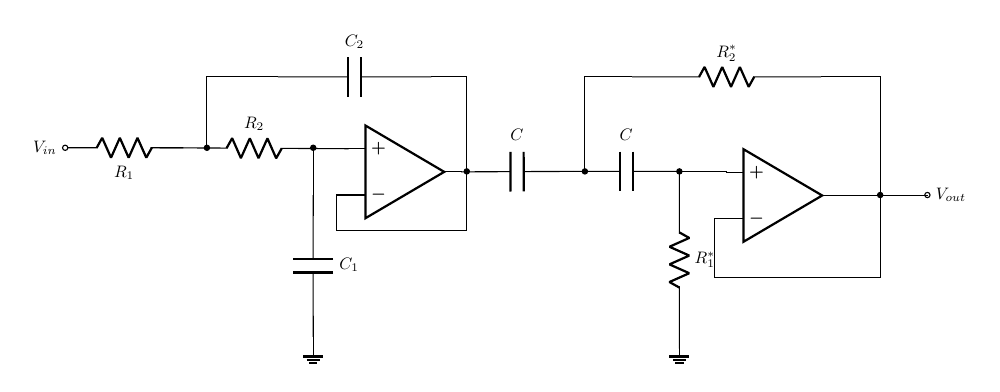
\begin{tikzpicture}[scale=0.6, transform shape]
				% Paths, nodes and wires:
				\node[op amp, yscale=-1] at (-14.81, 4.49){};
				\node[op amp, yscale=-1] at (-6.81, 3.99){};
				\draw (-20, 5) to[american resistor, l={$R_2$}] (-16, 4.98);
				\draw (-19.5, 5) to[american resistor, l={$R_1$}] (-22, 5);
				\draw (-10, 6.5) to[american resistor, l={$R_2^*$}] (-6, 6.5);
				\draw (-9, 4.5) to[american resistor, l={$R_1^*$}] (-9, 0.75);
				\draw (-17.5, 6.5) to[capacitor, l={$C_2$}] (-14.25, 6.5);
				\draw (-16.75, 4) to[capacitor, l={$C_1$}] (-16.75, 1);
				\draw (-13.62, 4.49) to[capacitor, l={$C$}] (-11.25, 4.5);
				\draw (-11.25, 4.5) to[capacitor, l={$C$}] (-9, 4.5);
				\draw (-9, 4.5) -- (-8, 4.5);
				\draw (-11.25, 4.5) -| (-11, 6.5) -- (-10, 6.5);
				\draw (-6, 6.5) -- (-4.75, 6.5) -| (-4.75, 4) |- (-5.62, 3.99);
				\draw (-8, 3.5) -- (-8.25, 3.5) -| (-8.25, 2.25) -| (-4.75, 3.99);
				\draw (-19, 5) -| (-19, 6.5) -- (-17.5, 6.5);
				\draw (-14.25, 6.5) -| (-13.5, 4.5);
				\draw (-16, 4) |- (-16.25, 4) -| (-16.25, 3.25) -- (-13.5, 3.25) -| (-13.5, 4.5);
				\draw (-16.75, 4) -| (-16.75, 5);
				\node[ground] at (-16.75, 1){};
				\node[ground] at (-9, 1){};
				\node[circ] at (-19, 5){};
				\node[circ] at (-16.75, 5){};
				\node[circ] at (-13.5, 4.5){};
				\node[circ] at (-11, 4.5){};
				\node[circ] at (-9, 4.5){};
				\node[circ] at (-4.75, 4){};
				\node[ocirc](N1) at (-22, 5){} node[anchor=east] at (N1.west){$V_{in}$};
				\node[ocirc](N2) at (-3.75, 4){} node[anchor=west] at (N2.east){$V_{out}$};
				\draw (-4.75, 3.99) -| (-3.75, 4);
			\end{tikzpicture}
		}
		\caption{Unity-Gain Sallen-Key Band-Pass Filter}
		\label{fig:Unity-Gain Sallen-Key Band-Pass Filter}
	\end{figure}
	
	{For	given $C_1$ and $C_2$, the resistor values for $R_1$ and $R_2$ are calculated through:
		\[
		R_{1,2} = \frac{a_1 C_2 \mp \sqrt{a_1^2 C_2^2 - 4 b_1 C_1 C_2}}{4 \pi f_c C_1 C_2}
		\]
		For	given $C$, the resistor values for $R_1^*$ and $R_2^*$ are calculated through:
		\[
		R_1^* = \frac{1}{\pi f_c C a_1}
		,
		R_2^* = \frac{a_1}{4 \pi f_c C b_1}	\]}
	
	\subsubsection*{Calculated Theoretical Resistor \& Capacitor Values for Band-pass Filters\footnote{See Appendix \ref{app:practical values} for practical resistor \& capacitor values.}}
	
	\begin{table}[h!]
		\centering
		
		\begin{tabular}{|c|c|c|c|c|c|c|}
			\hline
			$R_1$ & $R_2$ & $C_1$ & $C_2$ &$R_1^*$ & $R_2^*$ & $C$ \\
			\hline
			1.2 k$\Omega$ & 2.2 k$\Omega$ & 220 nF & 470 nF &47 k$\Omega$ & 27 k$\Omega$ & 220 nF \\
			\hline
		\end{tabular}
		\caption{Resistor and Capacitor values (20 Hz – 300 Hz)}
	\end{table}
	\begin{table}[h!]
		\centering
		
		\begin{tabular}{|c|c|c|c|c|}
			\hline
			Frequency Range & $R_1$ & $R_2$ & $R_3$ & $C$ \\
			\hline
			300 Hz – 1 kHz   & 3.3 k$\Omega$ & 10 k$\Omega$ & 3.9 k$\Omega$ & 100 nF \\
			1 kHz – 4 kHz    & 2.7 k$\Omega$ & 8.2 k$\Omega$ & 6.8 k$\Omega$ & 33 nF \\
			4 kHz – 10 kHz   & 2.2 k$\Omega$ & 6.8 k$\Omega$ & 1 k$\Omega$   & 15 nF \\
			10 kHz – 20 kHz  & 2.2 k$\Omega$ & 5.6 k$\Omega$ & 390 $\Omega$  & 10 nF \\
			\hline
		\end{tabular}
		\caption{Resistor and Capacitor values for 1st \ac{MFB} Filter}
	\end{table}
	
	\begin{table}[h!]
		\centering
		
		\begin{tabular}{|c|c|c|c|c|}
			\hline
			Frequency Range & $R_1$ & $R_2$ & $R_3$ & $C$ \\
			\hline
			300 Hz – 1 kHz   & 15 k$\Omega$ & 47 k$\Omega$ & 15 k$\Omega$ & 10 nF \\
			1 kHz – 4 kHz    & 3.3 k$\Omega$ & 10 k$\Omega$ & 6.8 k$\Omega$ & 10 nF \\
			4 kHz – 10 kHz   & 2.7 k$\Omega$ & 8.2 k$\Omega$ & 1 k$\Omega$   & 6.8 nF \\
			10 kHz – 20 kHz  & 1.8 k$\Omega$ & 5.6 k$\Omega$ & 330 $\Omega$  & 6.8 nF \\
			\hline
		\end{tabular}
		\caption{Resistor and Capacitor values for 2nd \ac{MFB} Filter}
	\end{table}
	
	
	
	\subsection{Gain Controller}
	\noindent
	\begin{minipage}{0.48\textwidth}
		\centering
		\begin{circuitikz}
			% Op-amp
			\node[op amp] (opamp) at (0.44, 4.49) {};
			
			% Input resistor
			\draw (-4.5, 5) to[american resistor, l={$R$}] (-0.38, 4.98);
			
			% Feedback resistor (variable)
			\draw (-0.75, 6.25) to[variable american resistor, l={$kR$}] (2.25, 6.25);
			
			% Feedback wiring
			\draw (-0.75, 6.25) -- (-1, 6.25) -| (-1, 5);
			\draw (-0.75, 4) -- (-1, 4) -| (-1, 2.75);
			
			% Output connection
			\draw (1.63, 4.49) -| (2.5, 4.5) -- (2.5, 6.25) -- (2.25, 6.25);
			
			% Input/output nodes
			\node[ocirc](N1) at (-4.5, 5){} node[anchor=east] at (N1.west){$V_{in}$};
			\draw (2.5, 4.49) -| (2.75, 4.5);
			\node[ocirc](N2) at (2.75, 4.49){} node[anchor=west] at (N2.east){$V_{out}$};
			
			% Ground and connection dots
			\node[circ] at (-1, 5) {};
			\node[circ] at (2.5, 4.5) {};
			\node[ground] at (-1, 2.75) {};
		\end{circuitikz}
		\captionof{figure}{Gain Controller}
		\label{fig:GainController}
	\end{minipage}%
	\hfill
	\begin{minipage}{0.48\textwidth}
		\[
		\frac{V_{in}-0}{R} = \frac{0 - V_{out}}{kR}
		\]
		\[
		V_{out} = -kV_{in}
		\]
	\end{minipage}
	\subsection{Adder \& Gain Controller}
	\noindent
	\begin{minipage}{0.48\textwidth}
		\centering
		\begin{circuitikz}[scale=0.9,transform shape]
			% Paths, nodes and wires:
			\node[op amp] at (0.44, 4.49){};
			\draw (-0.75, 6.25) to[variable american resistor, l={$kR$}] (2.25, 6.25);
			\draw (-0.75, 6.25) -- (-1, 6.25) -| (-1, 5);
			\draw (-0.75, 4) -- (-1, 4) -| (-1, 2.75);
			\draw (1.63, 4.49) -| (2.5, 4.5) -- (2.5, 6.25) -- (2.25, 6.25);
			\draw (2.5, 4.49) -| (2.75, 4.5);
			\node[ocirc](N1) at (2.75, 4.49){} node[anchor=west] at (N1.east){$V_{out}$};
			\node[circ] at (-1, 5){};
			\node[circ] at (2.5, 4.5){};
			\node[ground] at (-1, 2.75){};
			\draw (-0.75, 4.98) |- (-1, 5) -- (-1.75, 5) -- (-2.5, 5) -| (-2.5, 6.5) -- (-2.5, 3.25);
			\draw (-6, 6.5) to[american resistor, l={$R$}] (-2.5, 6.5);
			\draw (-6, 5.5) to[american resistor, l={$R$}] (-2.5, 5.5);
			\draw (-6, 4.5) to[american resistor, l={$R$}] (-2.5, 4.5);
			\draw (-6, 3.5) to[american resistor, l={$R$}] (-2.5, 3.5);
			\draw (-6, 2.5) to[american resistor, l={$R$}] (-2.5, 2.5);
			\draw (-2.5, 3.25) -| (-2.5, 2.5);
			\node[ocirc](N2) at (-6, 6.5){} node[anchor=east] at (N2.west){$V_1$};
			\node[ocirc](N3) at (-6, 5.5){} node[anchor=east] at (N3.west){$V_2$};
			\node[ocirc](N4) at (-6, 4.5){} node[anchor=east] at (N4.west){$V_3$};
			\node[ocirc](N5) at (-6, 3.5){} node[anchor=east] at (N5.west){$V_4$};
			\node[ocirc](N6) at (-6, 2.5){} node[anchor=east] at (N6.west){$V_5$};
			\node[circ] at (-2.5, 5.5){};
			\node[circ] at (-2.5, 4.5){};
			\node[circ] at (-2.5, 3.5){};
		\end{circuitikz}
		
		\captionof{figure}{Adder and Gain Controller}
		\label{fig:Adder and Gain Controller}
	\end{minipage}%
	\hfill
	\begin{minipage}{0.4\textwidth}
		
		\[ \sum_{i=1}^{5} \frac{V_i-0}{R} = \frac{0-V_{out}}{kR}
		\]
		\[V_{out}=-k\sum_{i=1}^{5} V_{i}
		\]
		
	\end{minipage}
	
	\subsection{\ac{LED} Display}
	
	\begin{figure}[H]
		\centering
		\includegraphics[width=0.8\linewidth]{lm3915_cropped}
		\caption{Circuit connection for \ac{LED} display}
		\label{fig:led}
	\end{figure}
	
	\subsection{Power Amplifier Circuit}
	\begin{figure}[H]
		\centering
		% Resize to fit page width
		\resizebox{0.9\textwidth}{!}{%
			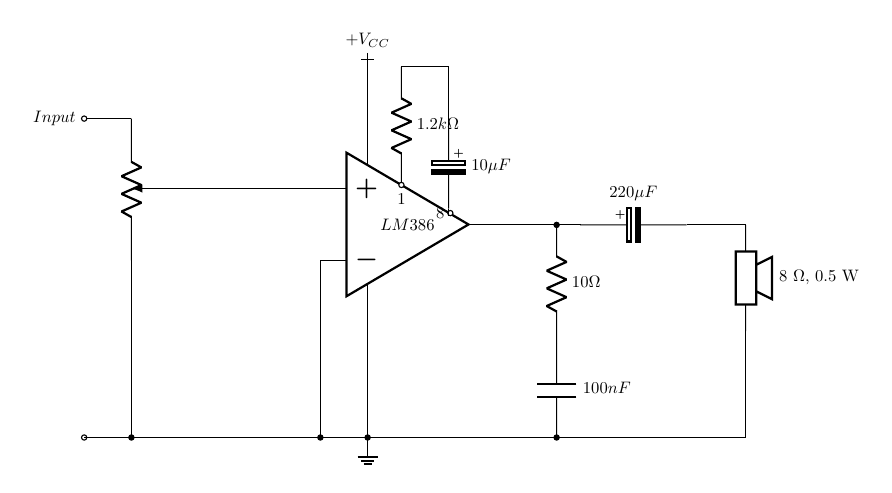
\begin{tikzpicture}[scale=0.6, transform shape]
				% Paths, nodes and wires:
				% Paths, nodes and wires:
				\node[op amp, xscale=1.55, yscale=-1.55](N1) at (-6.156, 4.509){} node[anchor=center] at (N1.text){$LM386$};
				\draw (1, 4.5) to[loudspeaker, l={8 $\Omega$, 0.5 W}] (1, 2.25);
				\draw (-12, 6.75) to[american resistor] (-12, 3.75);
				\draw (-3, 4.5) to[american resistor, l={$10\Omega$}] (-3, 2);
				\draw (-6.285, 7.845) to[american resistor, l={$1.2 k\Omega$}] (-6.285, 5.345);
				\draw (-3, 2) to[capacitor, l={$100 nF$}] (-3, 0);
				\draw (-5.285, 6.595) to[ecapacitor, l={$10\mu F$}] (-5.285, 4.845);
				\draw (-2.5, 4.5) to[ecapacitor, l={$220 \mu F$}] (-0.25, 4.5);
				\draw (-12, -0) -- (1, -0) -| (1, 2.25);
				\draw (1, 4.5) -- (-0.25, 4.5);
				\draw (-2.5, 4.5) |- (-4.311, 4.51);
				\draw (-6.285, 7.845) -- (-5.285, 7.845) -| (-5.285, 6.595);
				\draw (-7, 5.75) -| (-7, 8);
				\draw (-7, 3.25) -| (-7, -0);
				\draw (-8, 3.75) -| (-8, -0);
				\draw (-12, 6.75) -- (-13, 6.75);
				\draw (-12, 3.75) -| (-12, -0);
				\node[ground] at (-7, -0){};
				\draw[-latex] (-8, 5.269) -- (-12, 5.269);
				\node[ocirc](N2) at (-13, 6.75){} node[anchor=east] at (N2.west){$Input$};
				\node[ocirc] at (-13, -0){};
				\node[circ] at (-12, -0){};
				\node[circ] at (-8, -0){};
				\node[circ] at (-7, -0){};
				\node[circ] at (-3, -0){};
				\node[circ] at (-3, 4.5){};
				\node[plain crossing](N3) at (-7, 8){} node[anchor=south] at (N3.north){$+ V_{CC}$};
				\draw (-12, -0) -- (-13, -0);
				\node[ocirc](N4) at (-6.285, 5.345){} node[anchor=north] at (N4.south){$1$};
				\node[ocirc](N5) at (-5.25, 4.75){} node[anchor=east] at (N5.text){$8$};
				\draw (-5.267, 4.692) -| (-5.285, 4.845);
			\end{tikzpicture}
		}
		\caption{Power Amplifier Circuit}
		\label{fig:Power Amplifier Circuit}
	\end{figure}
	
	
	\section{Component Selection (Main electronic components)}
	
	\begin{enumerate}
		\item\textbf{NE5532 Operational Amplifier}
		\begin{itemize}
			
			\item \textbf{Low Noise}: 5\,nV/$\sqrt{\text{Hz}}$ suitable for high-fidelity audio
			\item \textbf{Bipolar Input}: Ensures low offset and distortion in precision audio
			\item \textbf{Dual Channel}: Two \ac{Op Amp} per IC for compact design
			\item \textbf{High Slew Rate}: 9\,V/$\mu$s supports wide dynamic range
			\item \textbf{Wide Bandwidth}: 10\,MHz gain-bandwidth product for audio applications
			\item \textbf{Wide Supply}: $\pm3$\,V to $\pm20$\,V operation for design flexibility
			\item \textbf{High Drive Capability}: Can directly drive 600\,$\Omega$ loads
		\end{itemize}
		\item \textbf{LM3915 Dot/Bar Display Driver}
		\begin{itemize}
			\item Logarithmic 3 dB/step response for audio
			\item Direct \ac{LED} drive without current-limiting resistors
			\item Simple setup with minimal external components
			\item Over-voltage protection ($\pm$35V) on input
		\end{itemize}
		
		
	\end{enumerate}	
	
	
	
	\begin{minipage}[t]{0.48\textwidth}
		\centering
		\includegraphics[width=0.4\textwidth]{ne5532}
		\captionof{figure}{NE5532P Operational Amplifier}
	\end{minipage}
	\hfill
	\begin{minipage}[t]{0.48\textwidth}
		\centering
		\includegraphics[width=0.48\textwidth]{lm3914}
		\captionof{figure}{LM3915 Dot/Bar Display Driver}
	\end{minipage}
	
	
	\section{\ac{PCB} Design}
	We designed 4 separate \ac{PCB}s using Altium Designer. (Why 4 \ac{PCB}s?\footnote{See Appendix \ref{app:PCB Schematics}.})
	\begin{multicols}{2}
		\begin{figure}[H]
			\centering
			\includegraphics[width=0.8\linewidth]{pre}
			\caption{2D pathway of Pre Amplifier Circuit}
			\label{fig:pre}
		\end{figure}
		\begin{figure}[H]
			\centering
			\includegraphics[width=0.8\linewidth]{fil}
			\caption{2D pathway of Filter Circuit}
			\label{fig:fil}
		\end{figure}
		\begin{figure}[H]
			\centering
			\includegraphics[width=0.8\linewidth]{pow}
			\caption{2D pathway of Power Amplifier Circuit}
			\label{fig:pow}
		\end{figure}
		\begin{figure}[H]
			\centering
			\includegraphics[width=0.8\linewidth]{display}
			\caption{2D pathway of \ac{LED} Display Circuit}
			\label{fig:display}
		\end{figure}
		
	\end{multicols}
	\begin{figure}[H]
		\centering
		\includegraphics[width=0.43\linewidth]{pcb}
		\caption{Soldered \ac{PCB}s}
		\label{fig:pcb}
	\end{figure}
	
	
	\section{Enclosure Design}
	
	\begin{multicols}{2}
		\begin{figure}[H]
			\centering
			\includegraphics[width=\linewidth]{en5.jpg}
			\caption{Enclosure front view}
			\label{fig:Enclosure front view}
		\end{figure}
		\begin{figure}[H]
			\centering
			\includegraphics[width=\linewidth]{en2.jpg}
			\caption{Right side view}
			\label{fig:Side view1}
		\end{figure}
		\begin{figure}[H]
			\centering
			\includegraphics[width=\linewidth]{en3.jpg}
			\caption{Back view}
			\label{fig:Back view}
		\end{figure}
		\begin{figure}[H]
			\centering
			\includegraphics[width=\linewidth]{en4.jpg}
			\caption{Left side view}
			\label{fig:Left side view}
		\end{figure}
	\end{multicols}
    \begin{figure}[H]
        \centering
        \includegraphics[width=0.5\linewidth]{Final.png}
        \caption{Final product}
        \label{fig:placeholder}
    \end{figure}
	
	\newpage
	\section{Software Simulation and Hardware Testing}
	\subsection{Software Simulation (Using LTspice)}
	
	\begin{figure}[H]	\centering
		\includegraphics[width=1\linewidth]{sim}
		\caption{Circuit Diagram}
		\label{fig:sim}
	\end{figure}
	\begin{figure}[H]
		\centering
		\includegraphics[width=1\linewidth]{overall}
		\caption{Frequency Response of Each Filter}
		\label{fig:Frequency Response of Each Filter}
	\end{figure}
	\begin{figure}[H]
	
		\includegraphics[width=1\linewidth]{overall1}
		\caption{Overall Frequency Response}
		\label{fig:overall1}
	\end{figure}
	
	
	\subsection{Hardware Testing}
	\begin{multicols}{2}
		\begin{figure}[H]
			\centering
			\includegraphics[width=\linewidth]{hardware1}
			\caption{Breadboard implementation}
			\label{fig:hardware}
		\end{figure}
		\begin{figure}[H]
			\centering
			\includegraphics[width=\linewidth]{hardware2}
			\caption{\ac{PCB} testing}
			\label{fig:harware2}
		\end{figure}
	\end{multicols}
	
	
	
	
	
	\section{Conclusion \& Future Works}
	The \textbf{Five Band Audio Equalizer} successfully achieves its primary objective of dividing an input audio signal into five distinct frequency bands and allowing individual gain control for each band. Through the integration of pre-amplifier, band-pass filter, gain control, adder, and power amplifier stages, the system provides a fully analog audio equalization platform with real-time visual feedback using an \ac{LED} display. The implemented filters effectively cover the entire audible range from 20~Hz to 20~kHz, enabling fine-tuned tonal adjustment and improved sound clarity. Experimental testing confirmed that the circuit delivers stable operation with low distortion and noise, demonstrating the effectiveness of the NE5532 \ac{Op Amp} and LM3915 \ac{LED} display driver in high-fidelity analog applications.
	
	\textbf{Future development} of the project can focus on several enhancements. Firstly, the system can be expanded into a \textbf{stereo equalizer} by duplicating the current design for left and right audio channels, enabling complete two-channel sound processing for improved spatial audio experience. Secondly, designing a dedicated \textbf{power supply unit} with voltage regulation and filtering will ensure stable performance and minimize noise interference. Additional improvements could include integrating tone presets, miniaturized \ac{PCB} layouts, and incorporating protection circuits to increase durability and user convenience. These developments would transform the prototype into a fully functional and reliable consumer-grade audio equalizer system.
	
	
	\section{Contribution of Group Members}
	\begin{tabular}{|l|p{9cm}|} % p{6cm} allows auto line wrapping
		\hline
		\textbf{Student's Name (Index No.)} & \textbf{Contribution} \\
		\hline
		Tennakoon U.G.R.B. (230629R) & Filter calculations, \ac{PCB} design, Testing \& debugging, Soldering \\
		\hline
		Ratnayake R.M.S.H. (203548R) & \ac{PCB} design, Circuits design, Circuits simulation, Soldering \\
		\hline
		Shehan M.N.N. (230613M) & Breadboard implementation, Enclosure Design, Testing \\
		\hline
		Dissanayake R.K.T. (230164K) &  \ac{LED} display circuit design \& breadboard implementation, Testing, Assembling \\
		\hline
	\end{tabular}
	
	
	\section*{Acknowledgment}
	
	We would like to express our sincere gratitude to \textbf{Mr. Chanula Luckshan}, our project supervisor, for his continuous guidance and support throughout the development of the \textit{Five Band Audio Equalizer} project. His valuable suggestions at the early stages of circuit design and his assistance in identifying and correcting errors during \ac{PCB} and enclosure design were instrumental in achieving a successful outcome.
	
	We also wish to extend our appreciation to \textbf{Dr. Pranjeevan Kulasingham}, our Signals and Systems lecturer, for providing us with a comprehensive understanding of analog filter design principles, which formed the foundation for our filter implementation in this project.
	
	Our heartfelt thanks go to \textbf{Dr. Sampath Perera}, the module coordinator of EN2091 Laboratory Practice and Projects, for his overall supervision, encouragement, and for providing the necessary resources to complete this project effectively.
	
	Finally, we would like to acknowledge the support of all the \textbf{laboratory assistants} of the Department of Electronic and Telecommunication Engineering for their technical help, timely guidance, and assistance during the hardware testing and implementation stages.
	
	\begin{thebibliography}{1}
		\bibitem{TI2002}
		Texas Instruments, \emph{op Amps for Everyone Design Guide}, Rev. 8, Advanced Analog Products, SLOD006B, Aug. 2002. [Online]. Available: https://web.mit.edu/6.101/www/reference/op\_amps\_everyone.pdf
		
		\bibitem{TI:NE5532}
		Texas Instruments, “NE5532 — Dual, 30-V, 10-MHz, low-noise operational amplifier for audio applications,”  
		TI product page (Datasheet Rev. J), Jan. 27, 2015.  
		[Online]. Available: \url{https://www.ti.com/product/NE5532}  
		\bibitem{lm3915_datasheet}
		Texas Instruments. \emph{LM3915 Dot/Bar Display Driver Datasheet}, SNVS740C. Revised Mar. 2013. [Online]. Available: \url{https://www.alldatasheet.com/datasheet-pdf/view/558236/TI/LM3915.html}
		
		\bibitem{HomemadeCircuitsOpAmp}
		``Op Amp Preamplifier Circuits – For MICs, Guitars, Pick-ups, Buffers." \emph{Homemade Circuits}. Last Updated: Sept. 13, 2023. Available: \url{https://www.homemade-circuits.com/op-amp-preamplifier-circuits-for-mics-guitars-pick-ups-as-buffer/} 
		
		\bibitem{GaraipoomLM386}
		A. Garaipoom, ``LM386 Audio Amp Circuit – Build Small, Loud \& Battery-Friendly!," \emph{ElecCircuit.com}. Last Updated: Sept. 17, 2025. Available: \url{https://www.eleccircuit.com/lm386-audio-amplifier-circuit/} 
	\end{thebibliography}
	
	\newpage
	\section*{Appendix}
	\appendix
	
	\section{Practical Resistor \& Capacitor Values}\label{app:practical values}
	
	\begin{table}[h!]
		\centering
		
		\begin{tabular}{|c|c|c|c|c|c|c|}
			\hline
			$R_1$ & $R_2$ & $C_1$ & $C_2$ &$R_1^*$ & $R_2^*$ & $C$ \\
			\hline
			1.2 k$\Omega$ & 2.2 k$\Omega$ & 220 nF & 470 nF &47 k$\Omega$ & 27 k$\Omega$ & 220 nF \\
			\hline
		\end{tabular}
		\caption{Resistor and Capacitor values (20 Hz – 300 Hz)}
	\end{table}
	\begin{table}[h!]
		\centering
		
		\begin{tabular}{|c|c|c|c|c|}
			\hline
			\textbf{Frequency Range} & $R_1$ & $R_2$ & $R_3$ & $C$ \\ \hline
			300 Hz -- 1 kHz   & $2.7\,\text{k}\Omega$ & $10\,\text{k}\Omega$ & $10\,\text{k}\Omega$ & $100\,\text{nF}$ \\ \hline
			1 kHz -- 4 kHz    & $2.7\,\text{k}\Omega$ & $8.2\,\text{k}\Omega$ & $15\,\text{k}\Omega$ & $33\,\text{nF}$ \\ \hline
			4 kHz -- 10 kHz   & $2.2\,\text{k}\Omega$ & $6.8\,\text{k}\Omega$ & $1.2\,\text{k}\Omega$ & $15\,\text{nF}$ \\ \hline
			10 kHz -- 20 kHz  & $1.8\,\text{k}\Omega$ & $5.6\,\text{k}\Omega$ & $470\,\Omega$ & $10\,\text{nF}$ \\ \hline
		\end{tabular}
		\caption{Resistor and Capacitor values for 1st \ac{MFB} Filter}
	\end{table}
	\begin{table}[h!]
		\centering
		
		\begin{tabular}{|c|c|c|c|c|}
			\hline
			\textbf{Frequency Range} & $R_1$ & $R_2$ & $R_3$ & $C$ \\ \hline
			300 Hz -- 1 kHz   & $8.2\,\text{k}\Omega$ & $27\,\text{k}\Omega$ & $27\,\text{k}\Omega$ & $10\,\text{nF}$ \\ \hline
			1 kHz -- 4 kHz    & $2.2\,\text{k}\Omega$ & $8.2\,\text{k}\Omega$ & $15\,\text{k}\Omega$ & $10\,\text{nF}$ \\ \hline
			4 kHz -- 10 kHz   & $2.2\,\text{k}\Omega$ & $6.8\,\text{k}\Omega$ & $1.2\,\text{k}\Omega$ & $6.8\,\text{nF}$ \\ \hline
			10 kHz -- 20 kHz  & $1.5\,\text{k}\Omega$ & $3.9\,\text{k}\Omega$ & $390\,\Omega$ & $6.8\,\text{nF}$ \\ \hline
		\end{tabular}
		\caption{Resistor and Capacitor values for 2nd \ac{MFB} Filter}
	\end{table}
	\section{\ac{PCB} Schematics}\label{app:PCB Schematics}
    \subsection*{\ac{PCB} Partitioning as a Cost-Reduction Strategy}

The initial hardware implementation consisted of two printed circuit boards (\ac{PCB}s): a main circuit \ac{PCB} measuring 162.94~mm~$\times$~112.52~mm and a display \ac{PCB} measuring 119.63~mm~$\times$~58.67~mm. The total estimated manufacturing cost for this configuration was approximately \$20. 

To minimize fabrication costs, the final design was divided into four smaller modular \ac{PCB}s, each with dimensions below 100~mm~$\times$~100~mm. This allowed the design to qualify for low-cost prototyping services offered by \ac{PCB} manufacturers. Consequently, the total fabrication cost was reduced to \$8 (four boards at \$2 each). This partitioning approach resulted in a \textbf{60\% reduction in manufacturing cost}, achieved without compromising system functionality or performance.

    \begin{figure}[H]
        \centering
        \includegraphics[width=0.95\linewidth]{Sheet1_Sheet2_merged.pdf}
        \caption{Pre-Amplifer \& Filters }
        \label{fig:placeholder}
    \end{figure}
      \begin{figure}[H]
        \centering
        \includegraphics[width=0.95\linewidth]{Sheet3_display (2)_merged.pdf}
        \caption{Power Amplifier \& Display}
        \label{fig:placeholder1}
    \end{figure}
	
\end{document}
